\documentclass[a4paper,11pt]{article}
\usepackage[utf8]{inputenc}
\usepackage{textcomp}
\usepackage{lmodern}
\usepackage{listings}
\usepackage{graphicx}
\usepackage{listings}
\usepackage{color}
\definecolor{lightgray}{rgb}{0.9,0.9,0.9}
\definecolor{darkgray}{rgb}{0.4,0.4,0.4}
\definecolor{purple}{rgb}{0.65, 0.12, 0.82}
\usepackage{url}
\usepackage[top=3cm,bottom=3cm,left=3cm,right=3cm]{geometry}

\title{Royal Military Academy\\
	INFO-Y113 --- Management of Security: \\
	Concept Of Operations v2}

\author{DANHIER Piere, LECOCQ Alexis, NYAKI Loïc}

\begin{document}
\maketitle
\newpage
\tableofcontents

\newpage

\section{Introduction}
In recent years, cyber-security has become a primary concern for companies all over the world. No matter the size of the company, data often represent the heart of their business and whether the concern is the secrecy of intellectual property, or users' privacy, the theft of private data bears a huge cost for companies. Be it a monetary cost (lawsuits, fines) or a reputation cost (loss of trust, public outrage). In the case of government agencies, states secrets and other classified information could be stolen by a foreign nation, possibly leading to the loss of lives in conflict zones, loss of political leverage on the international scene, domestic political turmoil and scandals or simply public embarrassment.\\

When trying to protect these sensitive data, a common measure is be to physically isolate the network from the internet, by creating an \textit{air gap}. Acting this way ensures that the data from the network is inaccessible from the outside world. The main issue with this method is that inevitably, some external data or files will at some point need to be imported into the secure network, be it for software update, or simply because some files from the outside are necessary for the people working in the secure network. In that case, a manual import (via USB drive, by connecting and external laptop into the secure network, or by using some other data transfer device) will be necessary.\\

The problem with that method is that it can compromise the security of the secure network. For instance, the data that is manually transferred into the network may have been infected by a malware, or the secure network might already be infected by a virus. In both cases, there is a possibility for some malicious code to exfiltrate data, or to spread a virus outside, by secretly writing on the device that was originally used to import the data into the network.\\

As a consequence, we need to build a solution that prevents data leaks while allowing the transfer of files from the outside network into the secure network.

\section{Goals of this project}
We need to design a system that accomplishes two main goals :

\begin{enumerate}
\item{Isolate the content of a secure network from the outside world, while allowing data to be transferred from the outside world to that secure network.}
\item{Allow users of the system to be able to consult an administration web page, from the inside the secure network, in order to perform system management operations}
\end{enumerate}

For this project, the general solution is imposed and should be a data diode, which we will describe in section~\ref{sec:data-diode}.


\section{Objectives}
We identify the following objectives:
\begin{itemize}
\item{Build a file transfer functionality between the outside network and the secure network.}
\item{Ensure the integrity of the data during the file transfer, which means that the data that arrives in the secure network should be the same as the data that was sent from the outside.}
\item{Ensure data confidentiality: no data should be able to leave the the secure network. Keep in mind that the scope of our confidentiality concern is the secure network in relation to the outside world. Ensuring confidentiality between the users of the secure network itself is out of the scope of this project.}
\item{Ensure availability: The file transfer service and administration service should always be available to users. More precisely, an authorized person should always be able to transfer a file into the secure network, and an authorized user should always be able to access and operate the administration page.}
\end{itemize}
\section{Security requirements}
TODO : dans cette section, on va bien spécifier quelles sont les exigences demandées au niveau de la sécurité. C'était une des remarque qu'on avait fait à mon groupe l'an passé : on avait proposé une solution, mais on ne s'était pas basés sur des requirements pour faire notre choix quand à la solution. Donc ils nous avaient demandé : ok, vous utilisez cette technologie là, mais pourquoi? On répondait "ah ben ça va nous permettre ceci et celà". Et il nous disaient "mais c'est mis nulle part dans votre rapport que "ceci et cela" est une exigence.\\

Donc en gros, notre solution semblait arbitraire, car elle n'était pas basées sur une réponse à des exigences. Ce qu'ils voulaient, c'était qu'on identifie toutes les exigences au niveau de la sécurité, et qu'ensuite, on dise "voilà, selon les exigences X et Y qu'il nous faut respecter, nous décidons d'utiliser la solution B plutot que la solution A, car c'est la seule qui respecte toutes les exigences."

\section{Data Diode}
\label{sec:data-diode}
A data diode is a one-way data transfer system. It is composed of two server: one server communicates with the outside network and the other one communicate with the secure network. Moreover, these two servers are connected to one another through a single unidirectional fiber optics cable. The cable going in the other direction has been physically cut. As a consequence, data can only flow in one direction, which guarantees the "one-way" property.

\begin{figure}
	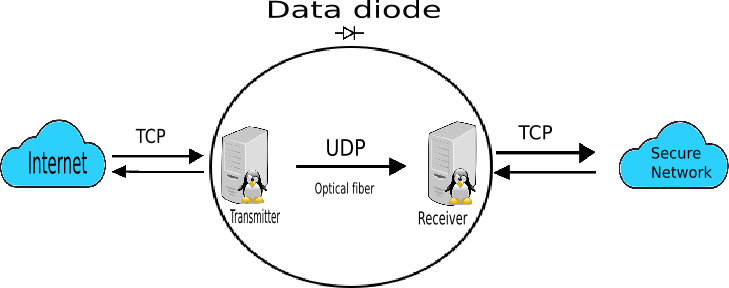
\includegraphics[scale=0.7]{img/network.png}
	\caption{High level architecture of a data diode.}
\end{figure}

\subsection{Applications}
With this data diode, we decided to keep things simple and to focus on proposing the two following services: a File Transfer service, as well as a data-diode management service. 
Other applications such as email management and web browsing will be considered for future versions of the data-diode.

\subsubsection{File Transfer}
The main application is a file transfer service that will enable files to be pushed from the outside network into the inside network, through the use of the File Transfer Protocol (FTP).

\subsubsection{Administration and Management}


\subsection{Architecture}
\subsubsection{Technical Aspects}
A data diode is composed of two servers linked by a one-way communication channel. The server, that we'll call the \textit{sender}, receives data from the external network with the TCP protocol. The second server, called the \textit{receiver}, uses the TCP protocol to send data to the secure network too. The same conclusion can then be applied to those data.\\

The one-way communication channel between the two sides of the data-diode forbids the use of a TCP based protocol (such as HTTP or FTP), as TCP requires bi-directional communication between two parties. As data between the two sides of the data-diode can only flow in one direction, we need data to be send over a protocol that doesn't require bi-directional communication. This can be done by using UDP for the communication between our two servers. The problem with UDP is that the sender cannot be sure that the receiver received the data or if the data is not corrupted. To mitigate this risk, we chose to send three times the packets of data.


\section{Users}

\section{Data Diode Administration and Management}
\end{document}